\chapter{Supervised Learning}
\label{ch:Supervised Learning}
\section{Introduction}
Supervised learning is a process of training a machine learning model, in which an algorithm is used to learn the mapping function $Y= F(X)$ from input to output. By and large, the desired output $Y$ might be hard to gather and consequently should be given by a human "Supervisor", yet the term applies in any event when the preparation set was gathered naturally. Most supervised learning algorithms depend on assessing a likelihood appropriation $p(y|x)$. We can do this basically by utilizing the most extreme probability assessment to track down the best boundary vector $\theta$ for a parametric spread model $p(y|x;\theta)$.

While preparing the model, information is generally parted in the proportion of $80:20$ for example $80\%$ as training data and the rest as testing data. The model gains from the training dataset as it were. We utilize distinctive AI algorithms, which we will talk about in detail in the following articles, to construct the trained model. By learning, it implies that the model will assemble some rationale of its own. At the test time, the data is taken from the rest $20\%$ of the dataset that the model has never seen, the model predicts the value and compares it with the original value to figure out the accuracy.

\section{Types of Supervised Learning}
\subsection{Classification}
It is a Supervised Learning task where outputs have characterized labels. For instance, Output – Purchase has characterized marks as $0 or 1$; $1$ states the client will buy and $0$ implies that the client will not buy. The objective here is to foresee discrete qualities having a place with a specific class and assess based on precision. It tends to be either paired or multi-class order. In paired order, the model predicts either $0 or 1$; however if there should be an occurrence of multi-class grouping, the model predicts more than one class.

Examples of classification learning algorithm
\begin{itemize}
    \item Stochastic Gradient Descent
    \item K-Nearest Neighbours
    \item Random Forest
    \item Support Vector Machine
\end{itemize}

\subsection{Regression}
It is a Supervised Learning task where outputs have constant labels; for example Output – wind speed does not have any discrete worth, however, is constant in the specific reach. The objective here is to foresee a worth as close to real yield as possible and afterward assessment is finished by figuring out an error. The more modest the loss the more noteworthy the exactness of the regression model. 

\begin{equation}
    \label{eq41}
    A \cdot x = b
\end{equation}

Curve fitting is the most essential of regression method, with polynomial and dramatic fitting bring about arrangements that come from settling the straight framework as in Eq. (\ref{eq41}). At the point when the model is not endorsed, at that point improvement techniques are utilized to choose the best model. There are different situations in a reality where we need some future forecasts like climate condition, deals expectation, promoting patterns, and so on, for such cases, we need some innovation which can make forecasts more precisely. So for such a case, we need Regression testing which is a measurable technique and utilized in AI and information science. The following are some applications of the Regression technique:

\begin{itemize}
    \item Regression measures the connection between the objective and the autonomous variable.
    \item It is utilized to discover patterns in information. 
    \item It assists with foreseeing genuine qualities.
    \item By tuning regression progress, we can unquestionably decide the main factor, the most insignificant factor, and the dependence of a parameter on other variables.
\end{itemize}

\textbf{Examples of classification learning algorithm}
\begin{itemize}
    \item Linear Regression
    \item Logistic Regression
    \item Polynomial Regression
    \item Support Vector Regression
    \item Decision Tree Regression
    \item Random Forest Regression
\end{itemize}

\section{Stochastic Gradient Descent with Momentum (SGDM)}
Training of a neural network by gradient descent method is similar to the training of any machine learning model; however, the neural network has a non-linearity that causes most of the loss function to become non-convex. Therefore, it is usually difficult to train a neural network that drives the loss to a minimum value. Additionally, stochastic gradient descent on non-convex loss function does not guarantee the convergence unlike in linear logistic regression case. Nevertheless, iterative gradient-descent-based optimization of appropriate convex function with proper initialization of parameters leads the gradient to converge to the minimum value. The stochastic gradient descent method is implemented in three steps as follows: 1. Loss and Cost Function, 2.Training, and 3.Forward and Backward propagation.

\subsection{Loss and Cost Function}
Neural network training is highly sensitive to the definition of the loss function. Intuitively, it seems that pass the training example from the network to get the output number and subtract it from the desire output number and square the result to find the loss. To exemplify, let us consider a single node neural network with the sigmoid activation function. The activation of this network is $ \hat{y}= \sigma \left(w^{T} x+b\right)$, where $\sigma(z)=\frac{1}{1+e^{-z}}$, x is an input, w and b are training parameters, $\sigma$ is a sigmoid activation function. The network output $\hat{y}$ should be close to the desired output $y$ for minimum loss. Therefore, as discussed earlier, the loss function is mention in Eq.(\ref{eq42}).

\begin{equation}
   \label{eq42}
   \mathcal{L}(\hat{y}, y)=\frac{1}{2}(\hat{y}-y)^{2}
\end{equation}

\begin{figure}
    \centering
        \begin{subfigure}[]
        \centering
        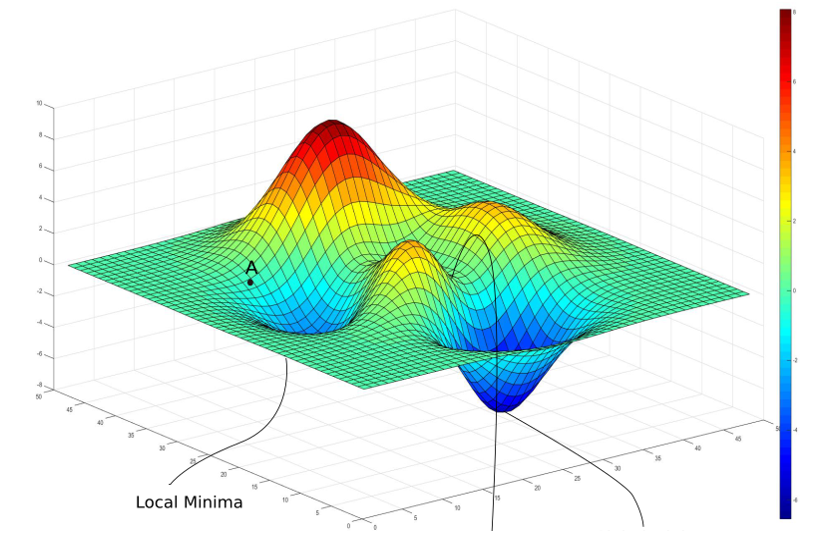
\includegraphics[width=0.45\textwidth]{Images/nonconvex.png}
        \end{subfigure}
        \rule{1.5px}{140px}
        \begin{subfigure}[]
        \centering
        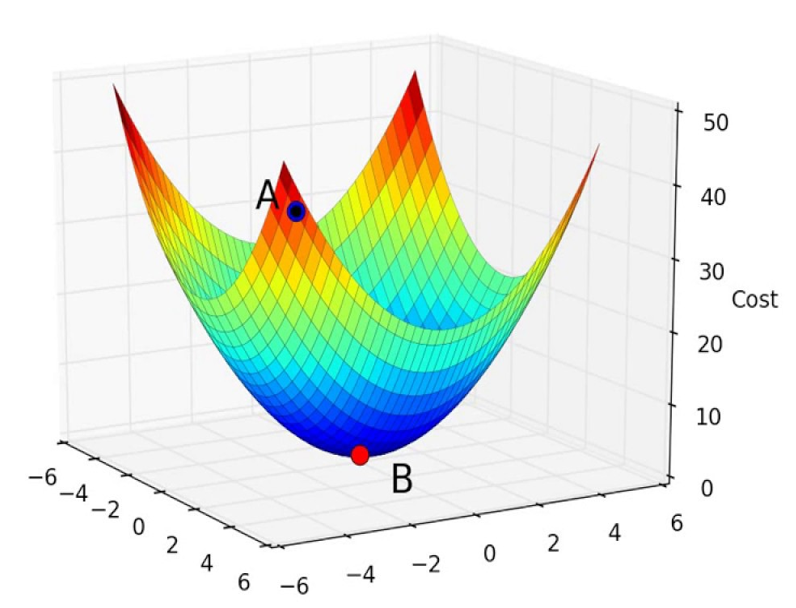
\includegraphics[width=0.45\textwidth]{Images/convex.png}
        \end{subfigure}
    \caption{Cost Function (a) Non-convex (b) Convex \cite{Convexity}}
    \label{costfunction}
\end{figure} 

The above loss function is generally used in linear regression problems, in contrast for a non-linear model the quadratic form of loss function becomes non-convex. Since there are multiple local minima as shown in Fig. \ref{costfunction}(a), gradient descent can not converge to a global minimum. In this case, a convex function that plays a similar role as an error function is used to minimize the discrepancy at the output. The convex loss function is defined as follows. 

\begin{equation}
    {L}(\hat{y}, y)=-(y \log \hat{y}+(1-y) \log (1-\hat{y}))
    \label{eq43}
\end{equation}

The justification for choosing the logarithmic loss function as shown in Eq. (\ref{eq43}) is as follows. When the desire output $y$ is $1$, the loss function become ${L}(\hat{y}, y)=-\log \hat{y}$. Therefore, the loss function tries to make $\hat{y}$ as large as possible, and the largest value that can be achieved of the $\hat{y}$ is $1$ because the highest possible value of the sigmoid activation function is $1$. On the other hand, when the desired output $y$ is $0$, the loss function is a change to ${L}(\hat{y}, y)=-\log (1-\hat{y})$ such that loss function pushes the $\hat{y}$ as small as possible.
 
The loss functions mentioned in Eq. (\ref{eq42}) \& (\ref{eq43}) are defined w.r.t single training example. However, the neural networks are trained on millions of training datasets, therefore the loss function is required to extend to use on multiple training data. The extension of the loss function is known as the cost function which is mentioned in Eq. (\ref{eq44}). The typical surface plot of this cost function is pictured in Fig. \ref{costfunction}(b).    

\begin{equation}
    J(\omega, b)=\frac{1}{m} \sum_{i=1}^{m} L\left(\hat{y}^{(i)}, y^{(i)}\right)=-\frac{1}{m} \sum_{i=1}^{m} [y^{(i)} \log \hat{y}^{(i)}+\left(1-y^{(i)}\right) \log \left(1 - \hat{y}^{(i)})\right]
    \label{eq44}
\end{equation}

Where, m is the number of training examples in dataset, and i is an index of the training example.  

\subsection{Training}
The stochastic gradient descent with momentum is one of the state-of-the-art algorithm in training neural networks. It works faster and better than the conventional gradient descent algorithm. To speed up the convergence, it uses a momentum. The momentum or velocity is defined by exponentially weighted averages of neural network parameters. It finds the moving averages of noisy data and bring them closer to the original values. As illustrated in Fig. \ref{movingaverage}, the yellow line is seems to be closer to the original function. The momentum of neural network parameters $w$ and $b$ are defined in Eq. (\ref{eq45}). The momentum parameter $\beta$ represent the number of values average at each iteration which can be derive by as follows $\frac{1}{1-\beta}$. Typically in learning the value of momentum parameter would be choose to 0.9, which tends it is averaging over last 10 values.

\begin{figure}
    \centering
    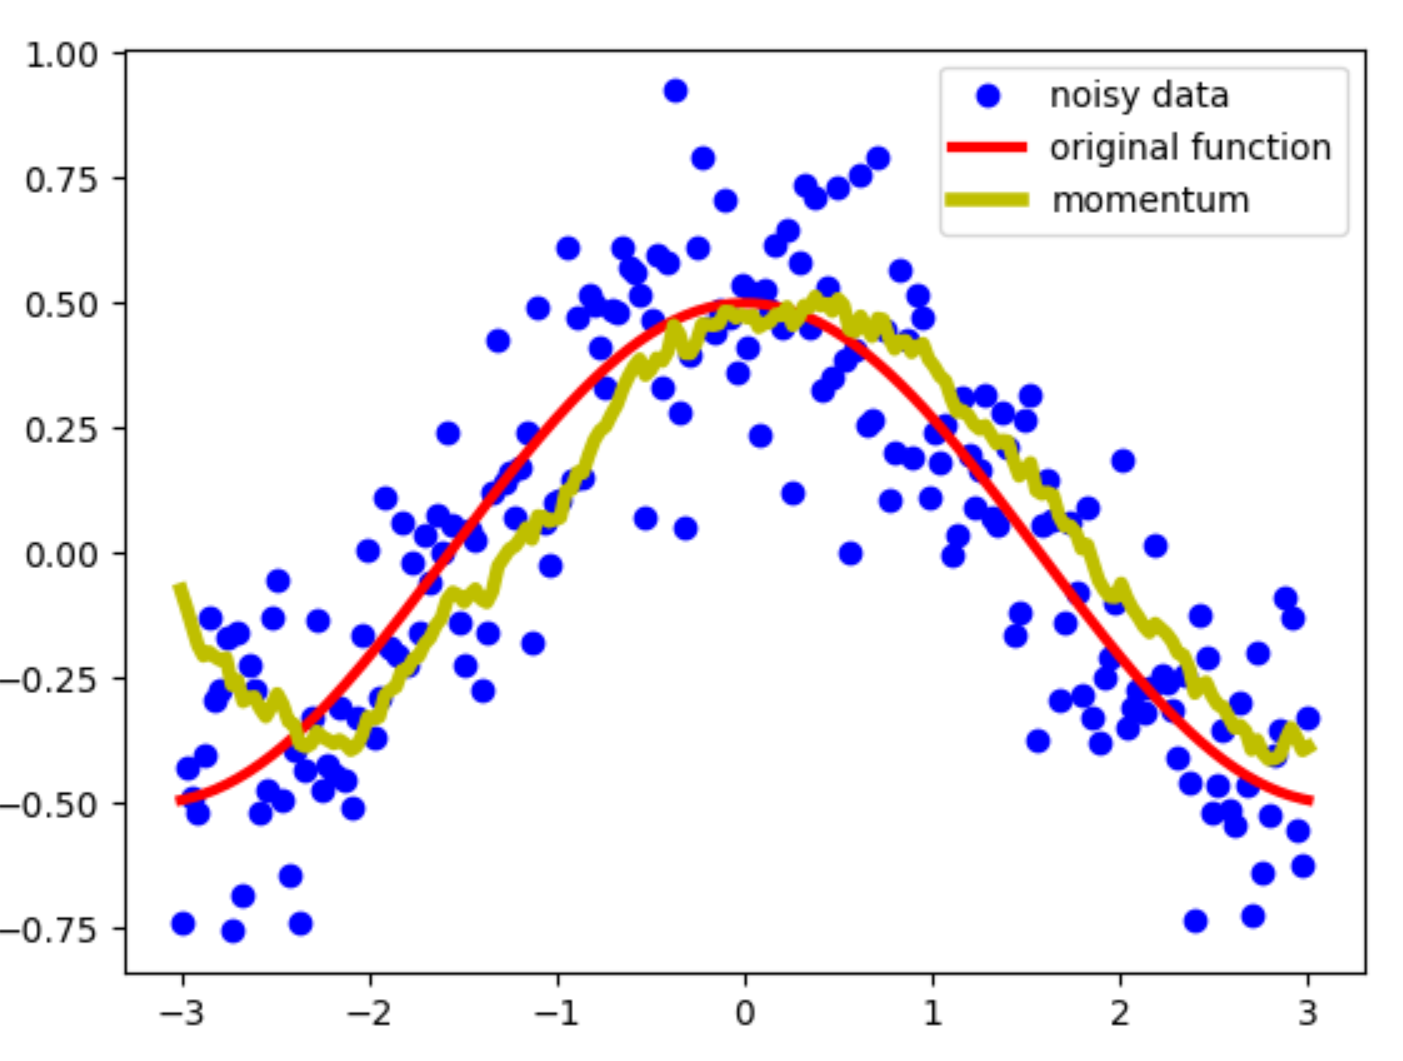
\includegraphics[width=0.55\textwidth]{Images/movingaverage.png}
    \caption{Exponentially Weighted Average of Noisy Data \cite{gradientdescent}}
    \label{movingaverage}
\end{figure} 

\begin{figure}
    \centering
    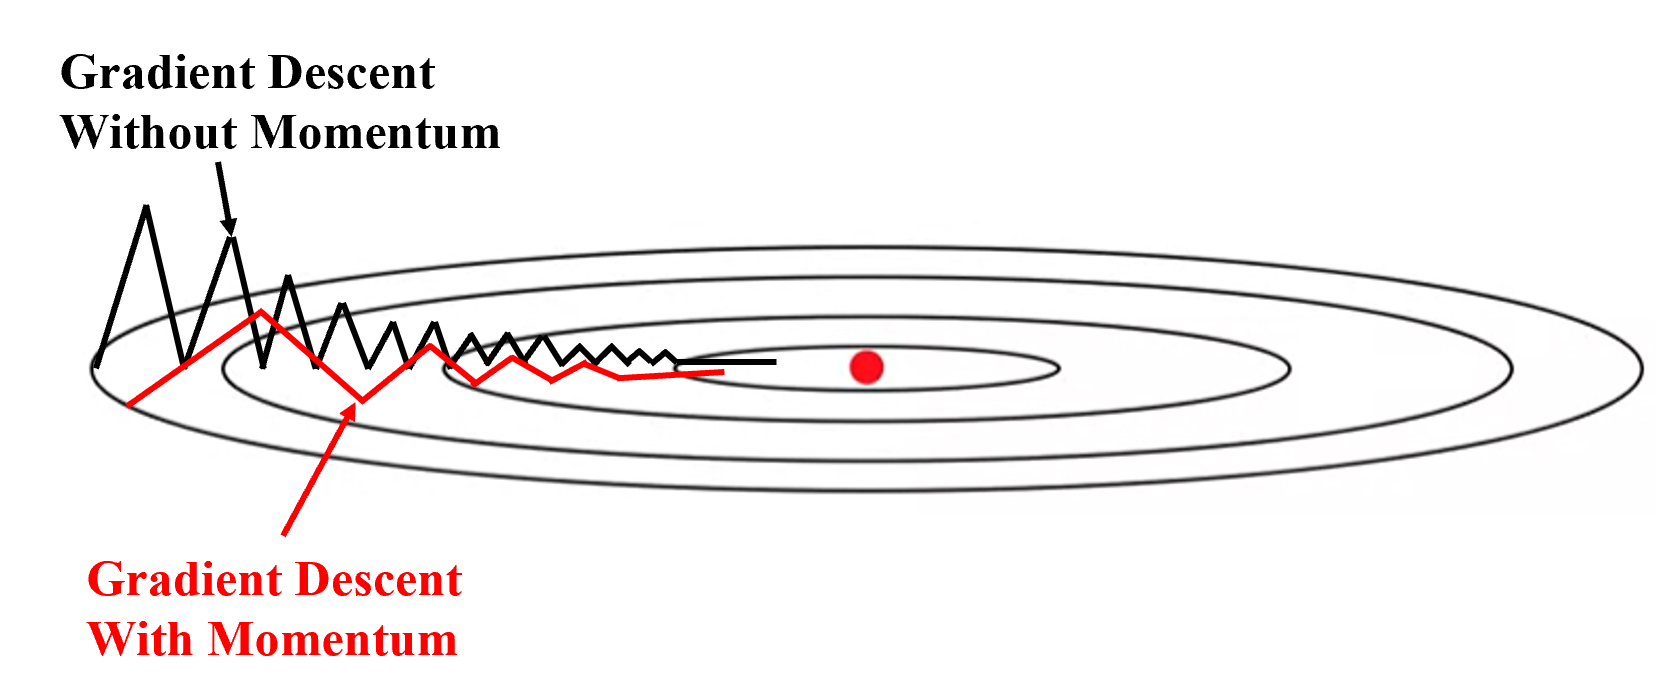
\includegraphics[width=0.55\textwidth]{Images/SGDM.png}
    \caption{Robustness of Stochastic Gradient Descent with Momentum}
    \label{SGDM}
\end{figure} 

\begin{equation}
    \begin{array}{l}
    \label{eq45}
     V_{d W}=\beta v_{d W}+(1-\beta) d W \\
     V_{d b}=\beta v_{d b}+(1-\beta) d b
    %W=W-\alpha v_{d W}, \quad b=b-\alpha v_{d b}
    \end{array}
\end{equation}

Where, $V_{d W}$ \& $V_{d b}$ are the momentum of weight and bias respectively, and $\beta$ is a momentum parameter.  

However, the bias is considerably high initially as shown in Fig. \ref{movingaverage}. The high bias value can be reduce by using bias correction term which is define as follow $\frac{V_{d W}}{1 - \beta^t}$. From the equation, it is inferred that up to certain numbers of iteration the bias correction reduces the bias because the denominator is smaller and as the number of iteration increases the denominator moves closer to $1$ that makes a little change in momentum. 

As mention earlier, the SGDM is robust compare to other gradient descent methods which can be justified from Fig. \ref{SGDM}. The black line, which represent the steps for simple gradient descent, is highly oscillatory; however, it average out the positive and negative values in oscillation which results in damping out the oscillation in vertical direction and pushes learning path towards the minima as represented by red line. The neural network parameters update after calculating momentum and bias correction is defined in Eq. (\ref{eq46}).  

\begin{equation}
    \begin{array}{l}
    \label{eq46}
     W=W-\alpha \cdot V_{d W} \\
     b=b-\alpha \cdot V_{d b}
    \end{array}
\end{equation}

Where, $\alpha$ is a learning rate of training which states the size of the step. 

\subsection{Forward and Backward Propagation}
In context to deep learning training, the back-propagation is a practice of fine-tuning neural network parameters based on the error from the previous iteration and forward propagation is associated with deriving the amount of error after perform tuning the neural network parameters. In the regression training, the parameters weight and bias are initialized and propagated forward to find the amount of loss at the output layer of the network. Further, the gradient of loss function w.r.t weights and biases are calculated at each layer in the backward direction. The flowchart of forward and backward propagation in stochastic gradient descent is illustrated in Fig. \ref{propogation}.             

\begin{figure}
    \centering
    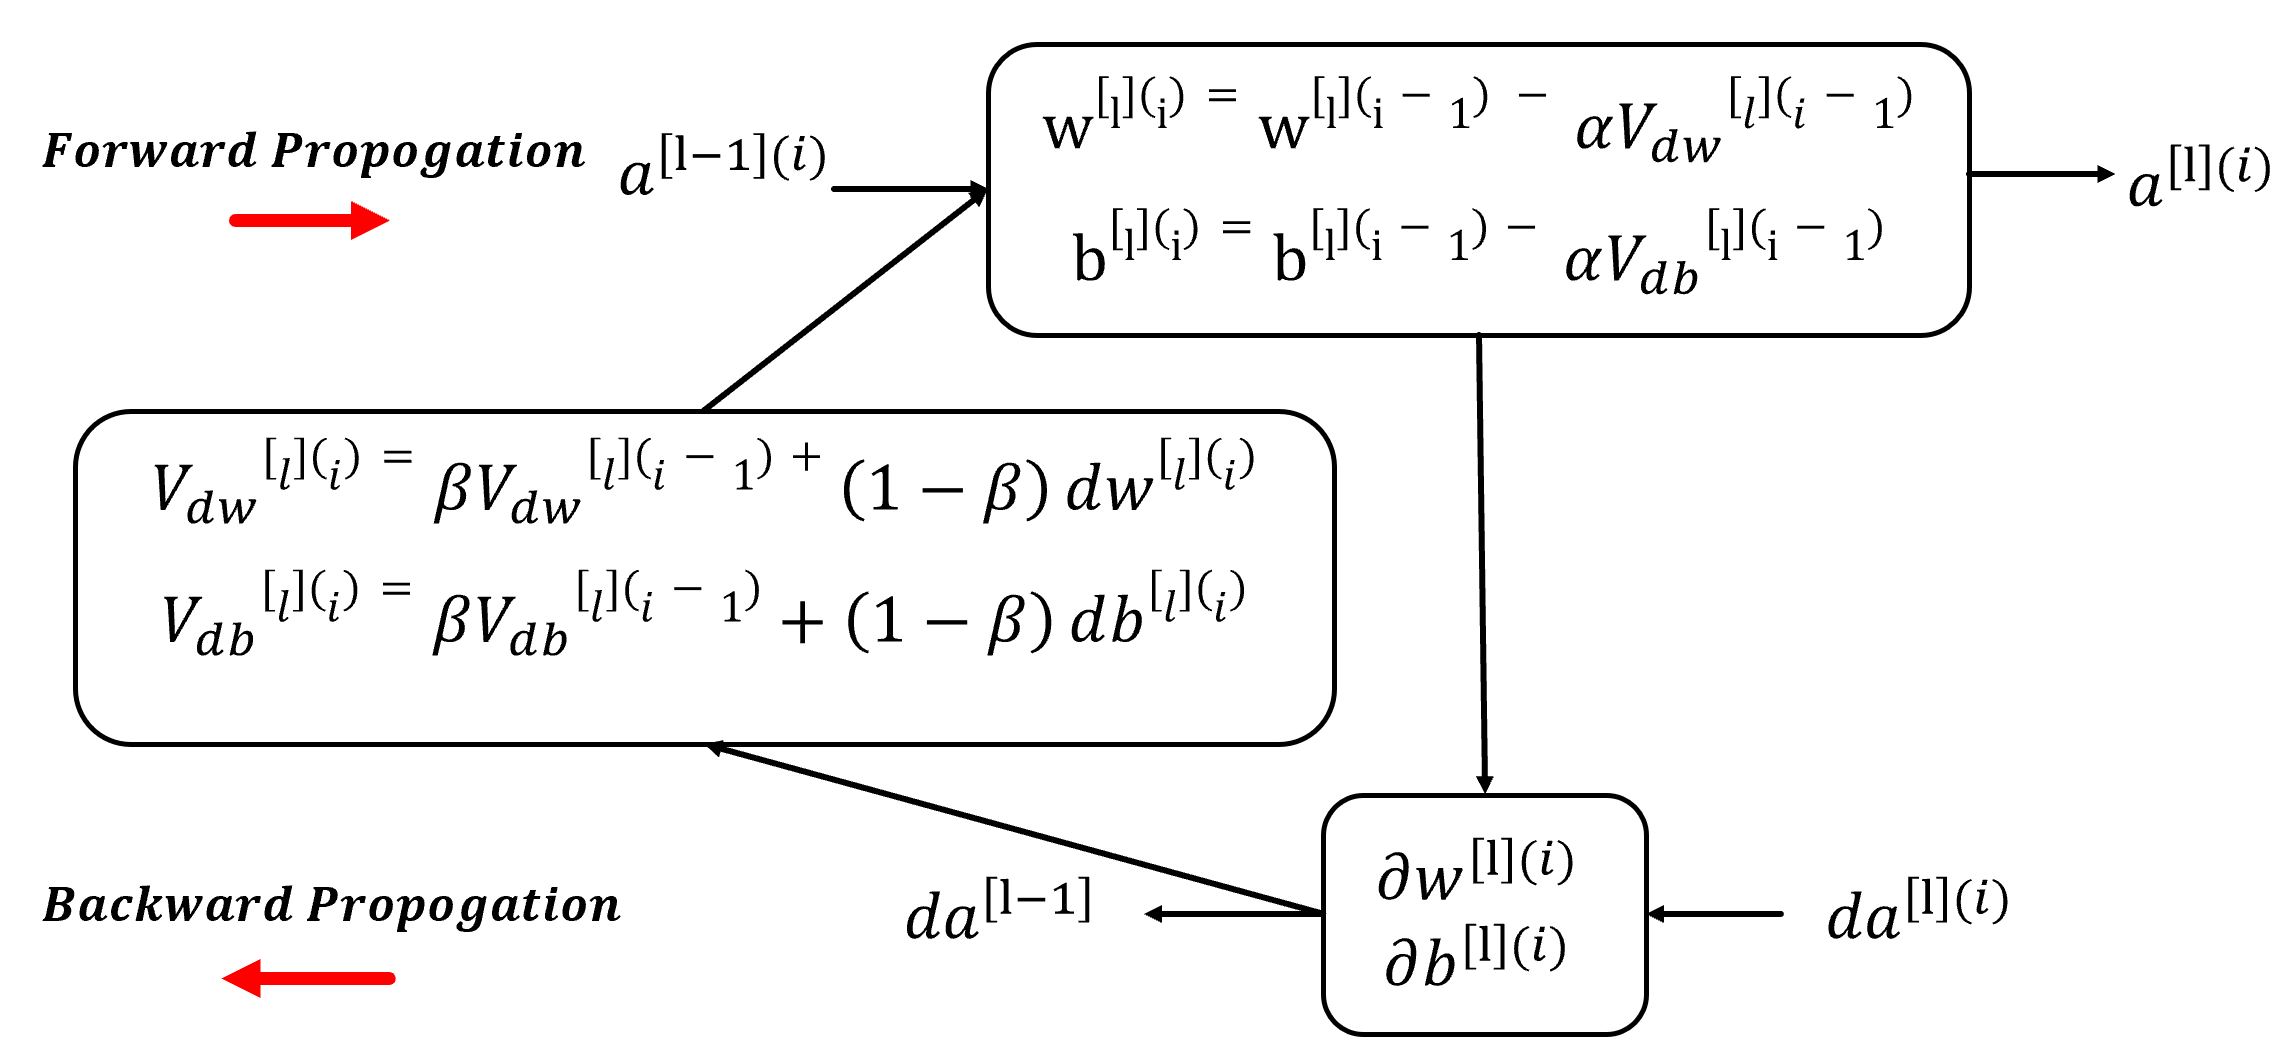
\includegraphics[width=0.95\textwidth]{Images/propogation.png}
    \caption{Flowchart of Forward and Backward Propagation}
    \label{propogation}
\end{figure} 

\section{YOLO algorithm}
YOLO algorithm predicts the class and bounding box of a detected object in a single run of the algorithm based on the regression method. The schematic of object detection in YOLO is shown in Fig. \ref{YOLO}. It uses features from CNN architecture to classify and detect objects. As illustrated in Fig. \ref{YOLO}, the output from the last convolutional layer of the base network passes through the soft-max layer to classify object categories with their precision. The same output is used for object detection. 

\begin{figure}
    \centering
    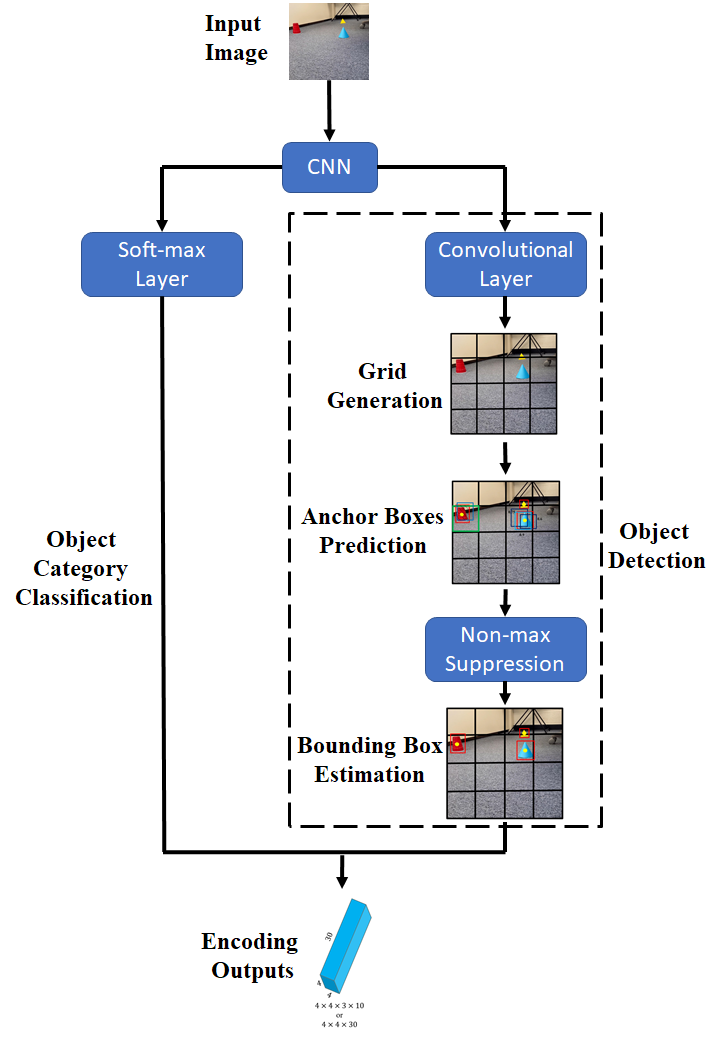
\includegraphics[width=0.9\textwidth]{Images/YOLO.png}
    \caption{YOLO Object Detection Pipeline}
    \label{YOLO}
\end{figure} 

In the detection head, the predefined grid established over the image as shown in the schematic. The object localization is performed to locate objects in each grid cells, which predicts multiple anchor boxes per grid. The number of anchor boxes that should be predicted per grid is predefined at the time of network design. The numbers of predicted anchor boxes for a cone are 4 as shown in Fig. \ref{IOU}, for example. These all predicted anchor boxes are associated with unique IoU (Intersection Over Union) values. From the non-max suppression layer, the anchor boxes with lower IoU filtered and highest IoU anchor boxes are assigned as the bounding box for corresponding objects. Finally, the coordinates of the centroid of the bounding boxes w.r.t image frame $(b_x,b_y)$, bounding boxes height $b_h$, and width $b_w$ and encoded in the output with the precision of object classification.

The YOLO object detector cannot learn the features of all bounding boxes from training data because there are millions of different sizes bounding boxes in the ground truth dataset which requires either a huge computational time or maybe impossible to train. Instead, the bounding boxes from the training dataset are grouped based on their IoU distance metric using the k-mean clustering algorithm. The estimation of anchor boxes is discussed in the following section.

\begin{figure}
    \centering
    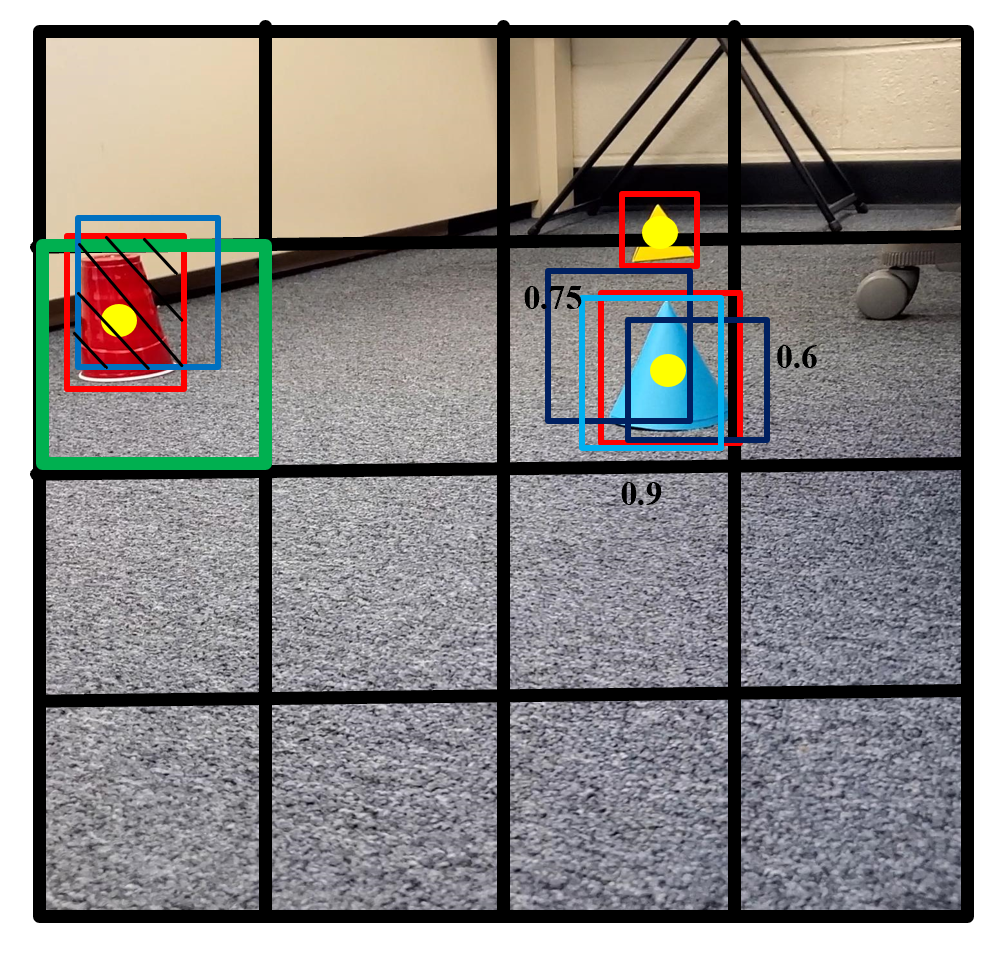
\includegraphics[width=0.5\textwidth]{Images/IOU.png}
    \caption{Anchor Boxes Estimation using IoU Distance Matrix}
    \label{IOU}
\end{figure} 

\section{Anchor Box Estimation}
Anchor box is an important entity in deep learning, particularly for object detection applications. The number, scale, and shape of the anchor box are hyper-parameters for neural network training which are tuned iteratively to achieve high accuracy. The anchor boxes are predefined from the ground truth dataset by performing anchor box estimation using the k-mean clustering technique. The network is trained to predict the probability and refinement of the corresponding predefined anchor box and the final feature map at the output represents the refined bounding box for each classified object. Since the use of the anchor boxes allows to detection of multiple objects in a single run, the object detector can be used for real-time applications. 

\begin{figure}
    \centering
    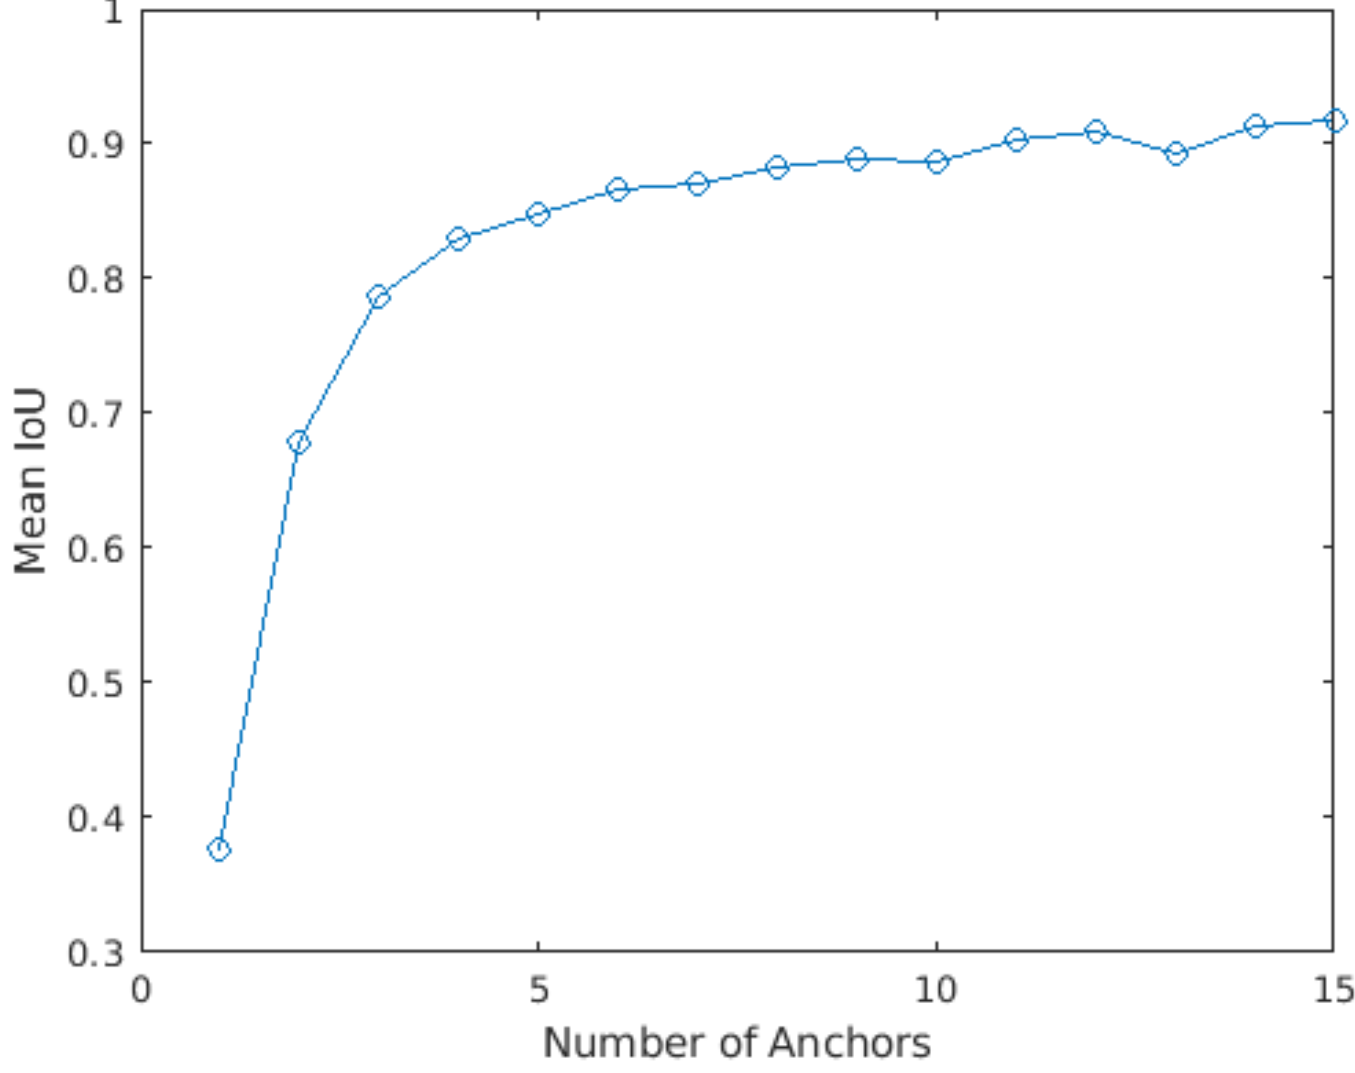
\includegraphics[width=0.5\textwidth]{Images/imperical.png}
    \caption{Trade off Between Number of Anchor Boxes and mean-IoU \cite{YOLO9000}}
    \label{imperical}
\end{figure}

The anchor box estimation from the training dataset is performed by use of the distance metric based on IoU because Euclidean distance metric-based estimation produces a larger error as the size of the boxes increases \cite{YOLO9000}.
Additionally, the IoU based anchor boxes estimation clusters together with the similar aspect ratio boxes that fit the ground truth data. 

As mentioned earlier, the number and mean-IoU required for the estimated anchor boxes are the hyper-parameter of the neural network. From the imperial result analysis, it has been seen that the number of anchors boxes is proportional to the mean-IoU of the boxes as represented in Fig. \ref{imperical}. The high value of mean-IoU improves the precision in the bounding box prediction and larger mean-IoU achieved by increasing the number of anchor boxes, however, a large number of anchor boxes leads to an increase in computation cost, and some cases may result in over-fitting.    
     
